\documentclass[12pt]{article}
\usepackage{latexsym}
\usepackage{amssymb,amsmath}
\usepackage[pdftex]{graphicx}
\usepackage{color}
\usepackage{epstopdf}


\topmargin = 0.1in \textwidth=5.7in \textheight=8.6in

\oddsidemargin = 0.2in \evensidemargin = 0.2in

\begin{document}

\begin{center}
COMPUTER SCIENCE 20, SPRING 2014 \\

\smallskip

Module \#19 (Undirected Graphs)
\end{center}
Author: Keenan Monks\\
Reviewer: Paul Handorff\\
Last modified: March 19, 2014

\medskip

\paragraph*{Executive Summary}
\begin{enumerate}

\item Undirected Graphs. An undirected (or simple) graph $G = (V,E)$ consists of a set of vertices $V$ and a set of edges $E$, which are unordered pairs of \textit{distinct} vertices. To indicate that there is an edge $e$ between some vertices $a,b \in V$ we write $e = \{a,b\}\in E$. The degree of a vertex, denoted as $deg(v)$, is the number of edges incident to that vertex.

\item The Handshaking Lemma. In a simple graph $G = (V,E)$, the sum of degrees of all vertices is equal to twice the number of edges:
\begin{center}
$2|E| = \sum\limits_{v \in V}  deg(v)$
\end{center}
\item Graph Types. A graph is \emph{complete} if there is an edge between all pair of vertices; the complete graph on $n$ vertices is written $K_n$. A graph is \emph{bipartite} if we can separate its vertices into two sets, such that there are no edges between vertices of the same set.

\item Undirected Graph Isomorphism. Two undirected graphs $G_1 = (V_1, E_1)$ and $G_2 = (V_2, E_2)$ are isomorphic if there is a bijective function $f: V_1 \rightarrow V_2$ such that
  $$\{a,b\} \in E_1 \Leftrightarrow \{f(a),f(b)\} \in E_2  $$

In other words, there is an edge between two vertices in $G$ if and only if there is an edge between their corresponding vertices in $H$. From this definition we can derive the following lemmas:
\begin{enumerate}
\item Isomorphic graphs have the same number of edges.
\item Isomorphic graphs have the same number of vertices.
\item If $G$ and $H$ are isomorphic, then the degree of any vertex in $G$ must be equal to the degree of its corresponding vertex in $H$.
\end{enumerate}
\end{enumerate}


\paragraph*{Small group problems}

\begin{enumerate}

\item Prove that if a simple graph has more than two nodes and is bipartite, then it cannot be complete. Draw the simple graph that has exactly two nodes and is both bipartite and complete.


\item We used directed graphs, not simple graphs, to represent relations because relations are inherently directional. If we tried to use simple graphs to represent relations, we would not be able to represent all relations. We can explore this by thinking about converting a simple graph into a digraph by replacing each undirected edge with a pair of opposite-pointing directed edges. If we did this, which of the following could we not possibly represent with digraphs constructed in this way? (Assume that we only consider graphs will at least one edge).
\begin{enumerate}
\item symmetric relations

\item reflexive relations

\item transitive relations

\item equivalence relations

\end{enumerate}

\item Determine which among the four graphs pictured below are isomorphic.  If two of these graphs are
isomorphic, describe an isomorphism between them.  If they are not,
give a property that is preserved under isomorphism such that one
graph has the property, but the other does not.

\begin{center}
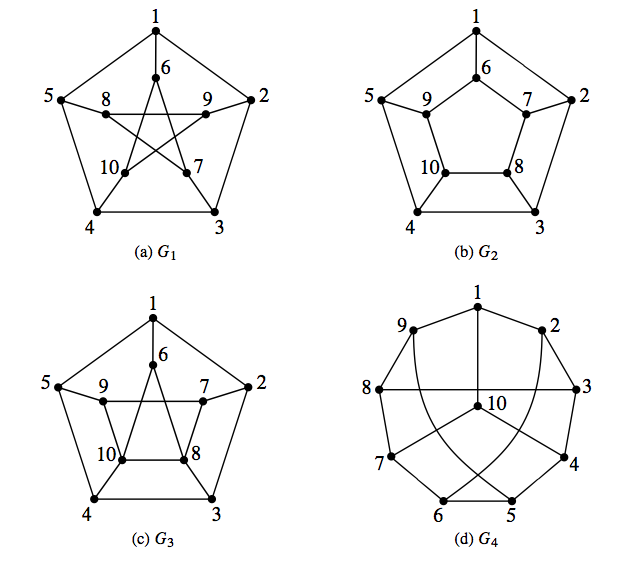
\includegraphics[scale=0.35]{all.png}
\end{center}

\item Prove that isomorphism of graphs is an equivalence relation.

\item Prove that any simple graph with at least two vertices has at least two vertices of the same degree.
\end{enumerate}

\end{document}
